The aim of this proposal is to (1) identify a set of principles for the analysis (formal, static,
  and dynamic) of communication protocols and
  their implementations in embedded systems; (2) implement these theoretical principles in tools usable by
  engineers developing such systems; and (3) use these tools in two real applications.
  In the first case study, we will formally, statically, and dynamically analyze networks
  of wireless sensor/actuator nodes deployed in the Southwest Experimental Garden
  Array (SEGA)~\cite{YamEtAl10,FliEtAl12}, a distributed facility for
  examining climatic, genetic, and environmental factors in plant ecology.
  The second case study will use the tools to formally verify and dynamically test the distributed coordination code of multiple autonomous ground and aerial robots in a lab setting.


\begin{figure}[!t]
  \centering
  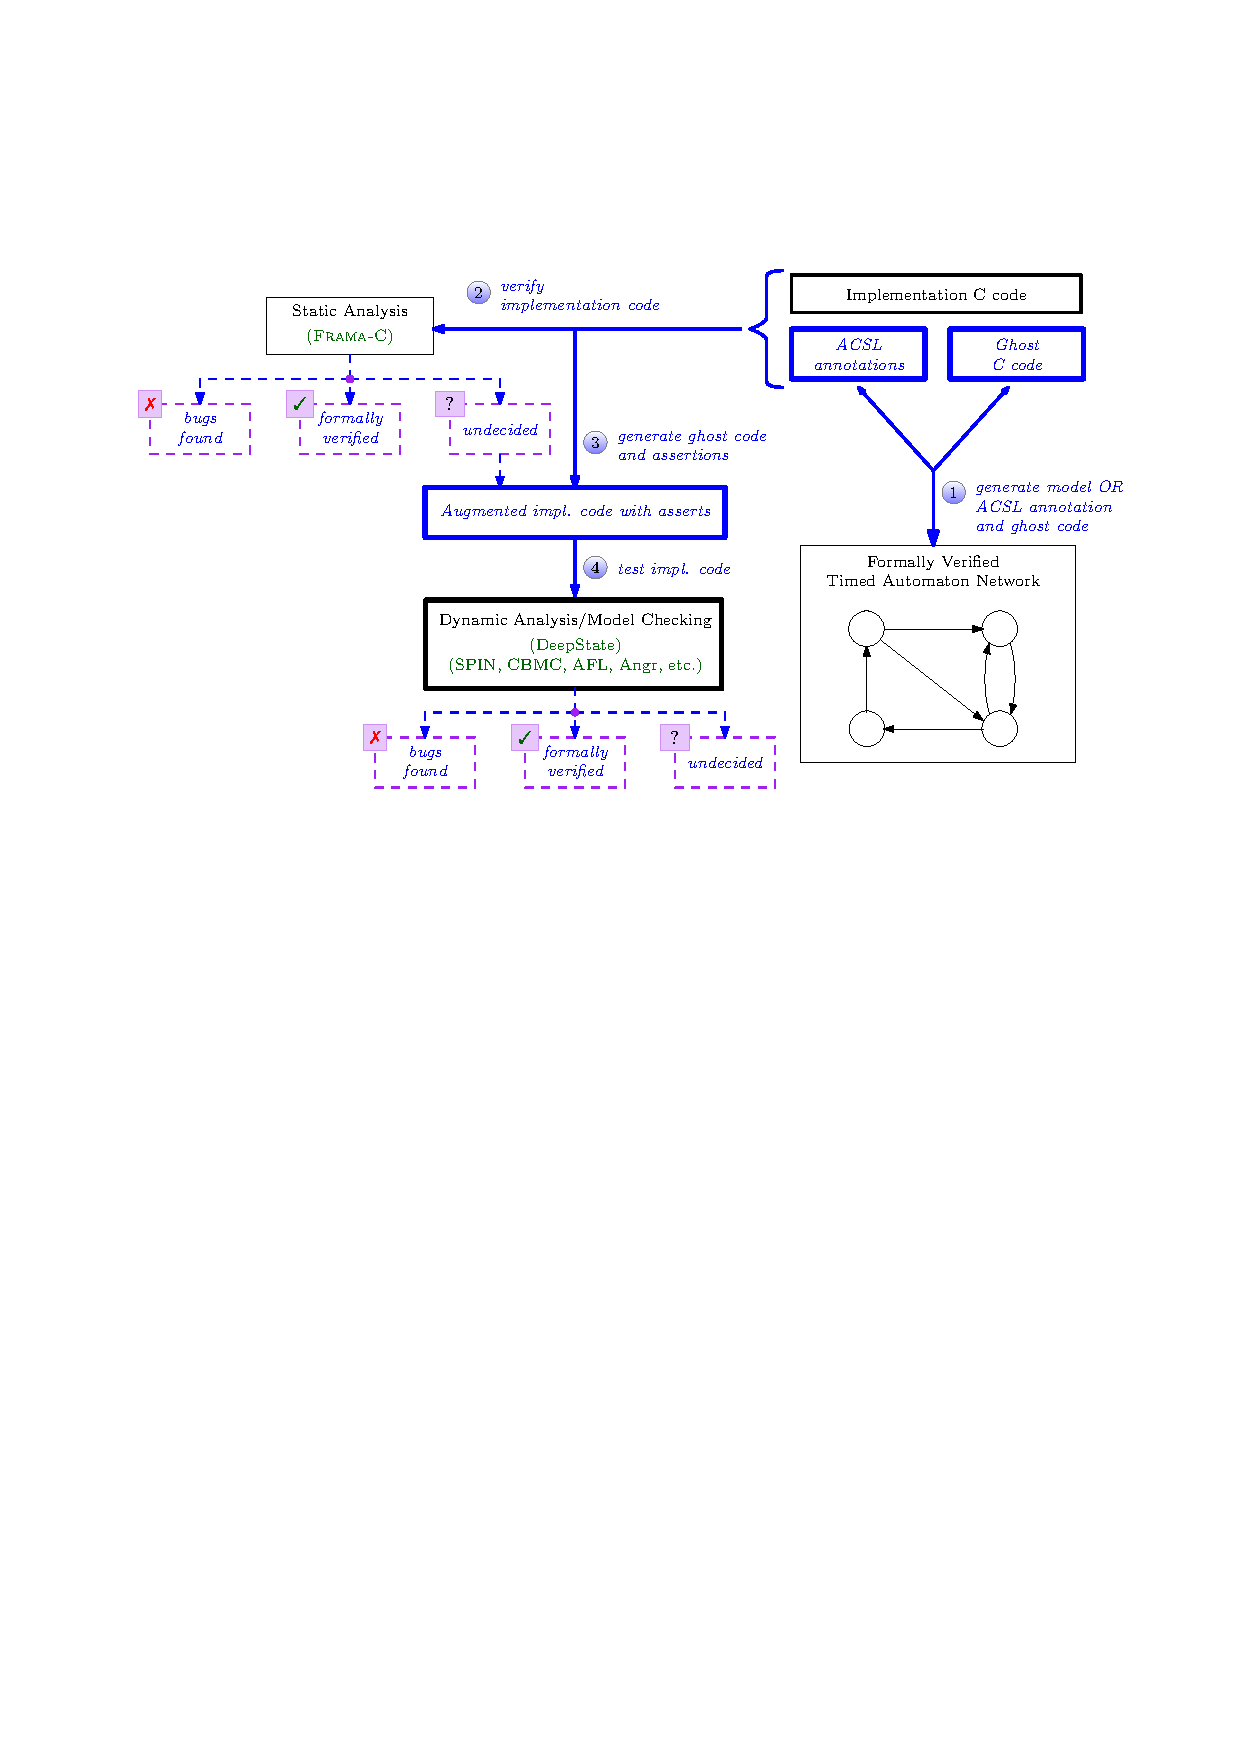
\includegraphics[width=.8\textwidth]{newoverview}
  \caption{Overview of the proposed research.}
  \label{fig:overview}
\end{figure}

Figure~\ref{fig:overview} shows the overall concept.  The core
open research problems addressed are represented by two sets of
arrows.  First, an engineering design, expressed as C code, is
provided, and annotated with correctness properties and information
about the expected environment (constraints on sensor values, etc.).
From this, code to apply advanced static analysis or generation of timed
automata (TA) models, can be automatically generated.  
Our goal is to certify whether the C code truly implements the
correctness properties in question:
\begin{enumerate}[labelsep=3pt,leftmargin=12pt]
\item First, the TA model can be used to check high-level properties
  of the design, ignoring many low-level implementation details.  If
  core timing properties are wrong, finding bugs in the implementation
  is best left until the basic design is correct.  However, this step
  may be skipped.
\item The implementation code with the \acsl annotations and ghost code
  is checked by a static analysis tool, such \framac.
  There are three possible outcomes:
  {\bf verified:} the implementation can be formally verified, which
  means that it meets the design specifications that can be checked statically;
  {\bf bugs found:} non-spurious bugs are found in the implementation, showing that
    it can violate the specification, and the bugs must be fixed; or
  {\bf undecided:} the static analysis tool is unable to prove or
  disprove correctness of the implementation, which will often be the case.
\item Finally, the focus of our efforts is a multi-pronged attempt to refute correctness (or increase our confidence
  in it) via dynamic analysis---automated test generation---and
  implementation-level model checking.
  Ghost code, additional runtime assertions, and needed test-harnesses are \emph{automatically generated} from the
  annotated code.
\item The augmented implementation code is then analyzed using the
  \deepstate~\cite{DeepState} framework, which serves as a front-end
  to highly scalable fuzzers, as well as to symbolic execution tools
  and explicit-state and SAT/SMT-based bounded model checkers that can
  detect more bugs at the cost of restricted applicability or scalability.  Generated test cases may
  prove the system faulty, or they may leave us more confident
  the system is correct.
\end{enumerate}

Our focus is on providing a unified specification method that can be
applied to source code itself, and on the dynamic analysis and
explicit-state and SAT/SMT bounded model
checking aspects of the approach.  We believe these approaches are
currently the most difficult to apply, and the most likely to
dramatically improve the ability to detect bugs in complex embedded
systems designs.

\paragraph{Principles:} Assuming that a communication protocol can in theory be described
as (probabilistic) timed automata~\cite{AD1994:TCS},
which satisfies temporal logic
formulas~\cite{BLM2017:LNCS}, and implemented as a set of
imperative programs that realize these timing constraints and other
correctness conditions, we ask:
\begin{itemize}[labelsep=3pt,leftmargin=12pt]
\item Given a set of annotated programs, how can we best automatically
  find bugs in those programs (and, in some circumstances, for some
  properties, prove correctness), based on the annotated
  specification?
\item Can we generate a skelton of the timed automata model from 
  annotated programs, in order to facilitate analysis of the design, 
  in order to increase adoption of design-level analysis by 
  traditional embedded systems developers? 
\end{itemize}
% REMOVED MENTIONS OF THE TOY LANGUAGE
%For the first problem, we will consider a toy imperative language with the
%usual control structures, unbounded integers, addresses, and
%non-recursive procedures.

Note that these problems differ considerably from the more studied,
but more limited, synthesis problem.  We are not assuming that
system development will involve first producing a formal model, then
using that model to automatically generate an implementation; rather,
we consider the typical real-world scenario, where modeling is a
separate activity, either undertaken after implementation due to
concerns about reliability, or an activity during design that only
indirectly informs the implementation.  That is, the more studied
problem is producing a runtime semantics for a model; we address the
problem of reconciling a runtime semantics with a model semantics,
without unrealistic burden on engineers.  We begin with the
implementation side, because while realtively few embedded systems
engineers currently use formal models, all must implement their
systems.  Furthermore, to the extent that developers do more rigorous
testing and analysis of their systems, they primarily use unit tests, simple
fuzzing, and static analysis.  Any method that aims to increase the
adoption of formal methods and more powerful automated test generation
approaches, including implementation-level model checking and symbolic
execution, is likely to be successful to the extent that it enters the
design and implementation process via this existing ``bridge to
engineers and developers.''


\paragraph{Tools:} We will focus on C code, using \deepstate~\cite{DeepState}
as a front-end for dynamic and implementation-level model checking approaches, and
\uppaal~\cite{uppaal} and
\prism~\cite{KNP2011:CAV} for the analysis of protocols; \framac will
provide a powerful static analysis framework, and we well adopt the
\acsl language developed for \framac as a basis for our specification language.  The primary open research questions here are numerous, and include:
% (1) how to handle C constructs that are not part of the toy language;
(1) how to extend existing specification languages to support timing and uncertainty;
(2) how to assign the same meaning to a specification construct in
  various contexts, ranging from fuzzing to symbolic execution to
  explict-state model checking to bounded model checking in the
  ``dynamic'' \deepstate world, and including a static context for
  \framac and a modeling conext for timed automata.
(3) how to handle intra-program parallelism;
(4) how to effectively translate a failed proof effort in \framac
  into a representation of a testing problem (to find counterexamples
  refuting that proof could be possible) in a dynamic setting; and
(5) how to ensure that the methods are sufficiently automatic
  and behave in ways engineers (not formal modeling, static, or dynamic
  analysis experts) will expect.

Our focus will be on \emph{practical} solutions, guided by the
embedded domain experts, rather than on purely theoretical approaches
that do not scale to real systems. Practical solutions here require
fundamental contributions to system and specification design and
semantics and static and dynamic analysis methods.